Contracts that give one party the \textbf{(1)} \textit{right} to buy or sell a certain security, target risk better and information. \textbf{(2)} Allow us to learn incredibly granular levels of information. \textbf{(3)} target risks better and incredibly specific \textbf{(4)} Put information in a more targeted way. 

\begin{multicols}{2}
\subsection{Put Option}
The right to sell an asset for a certain price at a certain time in the future.
\subsection{Call Option}
The right to buy an asset for a certain price at a certain time in the future.
\subsection{Long Position}
The option buyer or holder pays a premium and receives the right to buy or sell an asset.
\subsection{Short Position}
The option seller or writer receives a premium and has the obligation to deliver or purchase an asset.
\subsection{Evaluate Options at Expiry}
\begin{itemize}
    \item $S_t$: Spot price, asset trading at time $t$.
    \item $X$: Strike or exercise price. 
    \item $T$: Strike or expiration date.
    \item $C_t$: Price of a call option.
    \item $P_t$: Price of a put option.
\end{itemize}

\end{multicols}

\begin{figure}[H]
    \centering 
    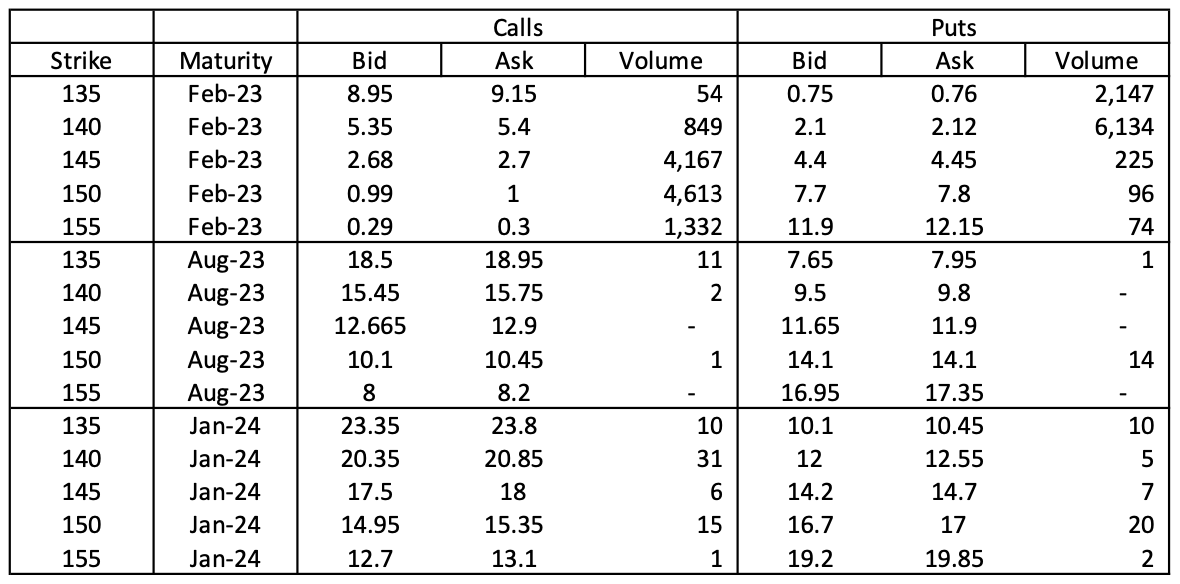
\includegraphics[width =0.65\textwidth]{Figure/option.png}
\end{figure}

\begin{multicols}{2}

From the Table above we can infer some information about the stock
\begin{itemize}
    \item The price of Call options decreases with increasing strike price, this is because people want to buy the stock at lower price instead of higher price, so I have to pay more for that right than the right to buy it at a more expensive price.
    \item The opposite is true for put options, where the right to sell at a lower price is less desirable
    \item For next-day expire option, if I know the price is not gonna change a lot between in one day for not very volatile stocks, and I know the right to buy this asset at say \$135 is \$9 today, it's probably gonna be \$9 tomorrow as well. Therefore, the value of the asset is most likely to be \$9 above \$135, which is around \$144 (or a range).
    \item options strictly has to be cheaper than the actual asset. It is also cheaper to buy an option if you think the price is going up.
\end{itemize}

A $\boxed{\textbf{Call option's value}}$ is:
\begin{gather*}
    C_T=\left\{
        \begin{array}{ll}
            \begin{split}
                S_T-X\hspace*{0.2cm}&\text{if}\hspace*{0.2cm}S_T>X\\
                0\hspace*{0.6cm}&\text{if}\hspace*{0.2cm}S_T\leq X\\
            \end{split}
        \end{array}
        \right.
\end{gather*}
\begin{figure}[H]
    \centering 
    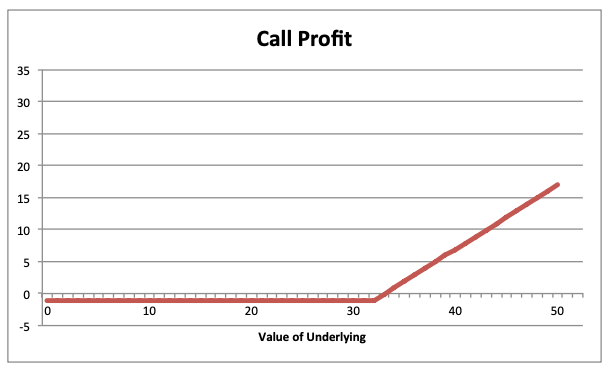
\includegraphics[width =0.4\textwidth]{Figure/call.png}
\end{figure}

A $\boxed{\textbf{Put option's value}}$ is:
\begin{gather*}
    P_T=\left\{
        \begin{array}{ll}
            \begin{split}
                0\hspace*{0.6cm}&\text{if}\hspace*{0.2cm}S_T\geq X\\
                X-S_T\hspace*{0.2cm}&\text{if}\hspace*{0.2cm}S_T< X\\
            \end{split}
        \end{array}
        \right.
\end{gather*}
\begin{figure}[H]
    \centering 
    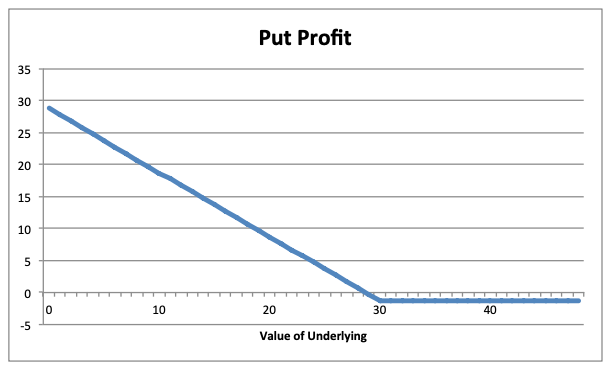
\includegraphics[width =0.4\textwidth]{Figure/put.png}
\end{figure}

\subsection{Option Strategies}
\subsubsection{Covered Calls}
\subsubsection{Protected Put}
\subsubsection{Bull Spread}
\subsubsection{Bear Spread}
\subsubsection{Butterfly Spread}
\subsubsection{Straddles/strangles}
\subsubsection{Strips/straps}

\subsection{Put-Call Parity}




\end{multicols}
